\chapter{Focus Before Diversification}

The interview opens with a familiar entrepreneurial premise: perhaps a founder should diversify beyond one or two things in order to become safer. The answer reverses that premise almost immediately. In this short School of Hard Knocks exchange, curated by LazyingArt LLC, diversification is not treated first as a portfolio virtue. It is treated as a question of timing, competence, and whether the first commercial engine has earned enough proof to justify spreading attention.

\section{The Question Behind Diversification}

The interviewer asks how important it has been, and how important it is for entrepreneurs in general, to diversify beyond one or two things. The hidden assumption is that more lines of business mean more stability. That assumption is common enough that it feels almost mathematical: do not put everything in one place; spread the risk.

But the lecture's first move is to notice that entrepreneurial diversification is not the same object as passive portfolio diversification. A founder is not merely allocating dollars across independent assets. A founder is allocating time, attention, judgment, sales energy, and operating discipline.

We can write the distinction schematically as
\begin{equation}
\text{financial diversification}
\neq
\text{founder attention spread}.
\end{equation}
The equation is not lecture notation; it is a compact way to preserve the spoken distinction. In a portfolio, spreading capital may reduce exposure. In an operating business, spreading the founder too early may reduce competence.

\subsection{Question \& Answer}

\paragraph{Question.}
Should entrepreneurs diversify beyond just one or two things?

\paragraph{Answer.}
The speaker's answer is abrupt: he does not think people should diversify. The reason is not that diversification can never be useful. The reason is that early diversification can become a way of limiting failures because the founder is not yet great at one thing.

The local lesson is therefore conditional:
\begin{equation}
\text{early diversification}
\neq
\text{automatic prudence}.
\end{equation}
The question asks about breadth. The answer insists on sequence.

\section{The Reversal: Focus Before Spread}

The speaker invokes, with an uncertain attribution, a Mark Cuban-style line: diversification is for people who are not great at one thing. We should keep the attribution loose, because the interview itself keeps it loose. The useful point is the mechanism behind the line.

If we call the first real business engine \(B_1\), then the issue is whether \(B_1\) has become strong enough to support expansion. Premature diversification replaces the harder question,
\begin{equation}
\text{How do we become excellent at } B_1?
\end{equation}
with the softer question,
\begin{equation}
\text{How do we avoid being fully exposed to } B_1?
\end{equation}
Those are different questions. One is about mastery. The other is about cushioning.

The speaker's criticism is that cushioning can arrive before competence. In that case the founder is not multiplying strength; he is distributing weakness across several fronts.

\section{A Minimal Model Of Founder Attention}

There is no blackboard mathematics in the source material, so the following is only a bookkeeping reconstruction of the interview logic. It helps us make precise why the answer treats founder diversification differently from passive investment diversification.

Let the founder have one unit of usable operating attention:
\begin{equation}
A = 1.
\end{equation}
If the founder divides that attention equally across \(n\) active projects, then the attention per project is
\begin{equation}
a_n = \frac{A}{n} = \frac{1}{n}.
\end{equation}
If the competence or execution quality of a project is an increasing function of focused attention, call it \(q(a)\), then spreading from one project to \(n\) projects changes the per-project operating quality from
\begin{equation}
q(1)
\quad \text{to} \quad
q\!\left(\frac{1}{n}\right).
\end{equation}
For \(n>1\), we have \(1/n < 1\), so an increasing quality function gives
\begin{equation}
q\!\left(\frac{1}{n}\right) < q(1).
\end{equation}
This is not a theorem about all businesses. It is the simple arithmetic of attention. If the founder is still learning one business, adding more fronts may reduce the attention available to the one front that most needs it.

\paragraph{Worked example.}
Suppose, only for illustration, that execution quality is proportional to founder attention:
\begin{equation}
q(a) = a.
\end{equation}
Then one focused business receives
\begin{equation}
q(1) = 1,
\end{equation}
while four simultaneous projects receive
\begin{equation}
q\!\left(\frac{1}{4}\right) = \frac{1}{4}
\end{equation}
per project. The reconstruction captures the speaker's warning: diversification can look like spreading risk, while in practice it may spread underdeveloped execution.

\begin{figure}
\centering
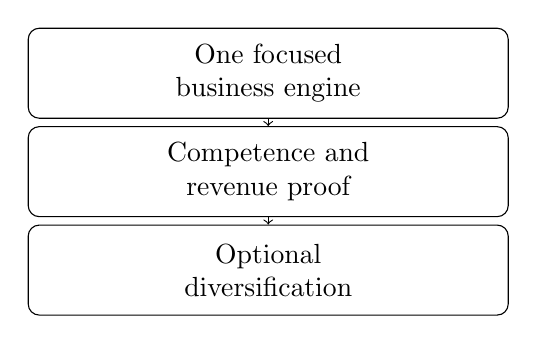
\begin{tikzpicture}
\node[draw, rounded corners, align=center, minimum width=2.4in, minimum height=0.45in] (focus) at (0,0) {One focused\\business engine};
\node[draw, rounded corners, align=center, minimum width=2.4in, minimum height=0.45in] (proof) at (0,-1.25) {Competence and\\revenue proof};
\node[draw, rounded corners, align=center, minimum width=2.4in, minimum height=0.45in] (option) at (0,-2.5) {Optional\\diversification};
\draw[->] (focus) -- (proof);
\draw[->] (proof) -- (option);
\end{tikzpicture}
\caption{A transcript-derived reconstruction of the speaker's sequence: focus first, prove the business, then consider diversification.}
\end{figure}

\section{The Revenue Anecdote}

The answer then turns from principle to personal sequence: the speaker says he did not start by diversifying. His solar company was doing more than ten million dollars in revenue before diversification entered the picture.

We can preserve the quantitative claim as
\begin{equation}
R_{\mathrm{solar}} > \$10{,}000{,}000.
\end{equation}
Here \(R_{\mathrm{solar}}\) denotes the reported revenue of the solar company. This is not a universal threshold. It is an anecdotal anchor. The point is not that every founder must wait for exactly ten million dollars. The point is that diversification came after a real commercial engine had already been demonstrated.

That changes the interpretation of diversification. Before proof, diversification may be a substitute for excellence. After proof, it may become optionality built on an operating base.

\section{Claim, Anecdote, And Mechanism}

It is useful to separate the three layers of the interview.

\paragraph{Claim.}
The speaker does not think people should diversify early.

\paragraph{Anecdote.}
He says he did not begin diversified; his solar company was already doing more than ten million dollars in revenue.

\paragraph{Mechanism.}
Diversification can limit failures when the founder is not yet great at one thing. In other words, the founder may be managing embarrassment or downside before mastering the engine that could create real upside.

A compact way to write the chapter's logic is
\begin{equation}
\text{focus}
\longrightarrow
\text{proof}
\longrightarrow
\text{optional diversification}.
\end{equation}
The arrow matters. The order is the argument.

\section{Summary}

The interview begins with diversification as the presumed virtue and ends with focus as the prior discipline. The speaker's answer is not a full theory of portfolio construction. It is a practical operating warning: a founder who has not become excellent at one thing may use diversification to limit failures rather than to compound strength.

The useful entrepreneurial rule is therefore not ``never diversify.'' It is more precise: do not let diversification arrive before competence, proof, and a working commercial engine.